\documentclass{article}
% Text %
%%%%%%%%
\usepackage[utf8]{inputenc}
\usepackage[spanish,es-lcroman]{babel}
% Images %
%%%%%%%%%%
\usepackage{graphicx}
\graphicspath{ {./images/} }
% Math packages %
%%%%%%%%%%%%%%%%%
\usepackage{amsmath}
\usepackage{amsthm}
\usepackage{amsfonts}
\usepackage{amssymb}
\usepackage{physics}
\usepackage{bbm}
\usepackage{mathrsfs}
% Math symbols %
%%%%%%%%%%%%%%%%
\DeclareMathOperator{\borel}{\mathscr{B}}
\DeclareMathOperator{\prob}{\mathbb{P}}
\DeclareMathOperator{\Expectation}{\mathbb{E}}
\DeclareMathOperator{\Variance}{\mathbb{V}}
\DeclareMathOperator{\Exponential}{\textnormal{Exp}}
\DeclareMathOperator{\normal}{N}
\DeclareMathOperator{\PhiDistribution}{\Phi}
\DeclareMathOperator*{\argmin}{\textnormal{argmín}}
\DeclareMathOperator{\characteristic}{\mathbbm{1}}
\DeclareMathOperator{\identity}{\textnormal{Id}}
\newcommand{\placeholderParameter}{-}
\newcommand{\symmetric}{\mathbb{S}}
\newcommand{\naturalnum}{\mathbb{N}}
\newcommand{\realnum}{\mathbb{R}}
\newcommand{\almostSurely}{\textnormal{ctp}}
\newcommand{\transpose}[1]{#1^T}
\newcommand{\brownian}{B}
\newcommand{\wiener}{W}
\newcommand{\events}{\mathcal{F}}
% Math environments %
%%%%%%%%%%%%%%%%%%%%%
\newtheorem{theorem}{Teorema}
\newtheorem{lemma}{Lema}
\newtheorem{corollary}{Corolario}
\newtheorem{property}{Propiedad}
\theoremstyle{definition}
\newtheorem{definition}{Definición}
\newtheorem{exercise}{Ejercicio}
% Lists %
%%%%%%%%%
\usepackage{enumitem}
% Counters %
%%%%%%%%%%%%

\title{Ejercicios para entregar}
\author{Pablo Brianese}

\begin{document}
\maketitle


% \begin{}
\begingroup
% Group variables %
%%%%%%%%%%%%%%%%%%%
\newcommand{\queueProcess}{(X_t)_{t \geq 0}}

\begin{exercise}
Consideremos un sistema que tiene un único servidor, que atiende a tasa $\mu > 0$, y los clientes llegan a tasa $\lambda > 0$.
Sea $X_t$ la cantidad de clientes que hay en la cola a tiempo $t$, con $t \geq 0$.
Notar que $\queueProcess$ es un proceso de Markov a tiempo continuo.
(Este modelo, llamado $M/ M / 1$, lo hemos charlado en la clase práctica 20 y 23).
\begin{enumerate}[label=\alph*), ref=\theexercise.\labelenumi]
    \item Probar que el proceso es recurrente positivo si y sólo si $\lambda < \mu$.
	Con lo cual, empezando con la cola vacía, el tiempo medio que tarda la cola en volver a vaciarse es finito si y sólo si $\lambda < \mu$.
	\item Asumiendo $\lambda < \mu$, calcular la proporción (asintótica) de tiempo que la cola está vacía.
\end{enumerate}
\end{exercise}

\begin{proof} a)
Comezamos analizando este proceso como lo hicimos en la clase práctica número 20.

% Cálculo de la matriz generadora del proceso %
%%%%%%%%%%%%%%%%%%%%%%%%%%%%%%%%%%%%%%%%%%%%%%%
% Nota 25 nov. 2020 teoría de proba  clase práctica 20.pdf %
%%%%%%%%%%%%%%%%%%%%%%%%%%%%%%%%%%%%%%%%%%%%%%%%%%%%%%%%%%%%
% Vamos a ver que \(\Expectation(T_0) < \infty\) si y solo si \(\lambda < \mu\).

% Si la cadena está en el estado 0, sólo puede saltar al 1; si está en un estado \(i > 0\), puede saltar a \(i - 1\) o a \(i + 1\).

% Si está en 0, salta al estado 1 cuando suena un reloj exponencial de parámetro \(\lambda\).
% Si se encuntra en un estado \(i > 0\), hay dos relojes exponenciales compitiendo, uno a tasa \(\lambda\), que indica la llegada de una persona y otra a tasa \(\mu\) que indica que una se va. 

% Usaremos los siguientes lemas sobre la distribución exponencial:
% \begin{enumerate}
% 	\item Si \(X \sim \Exponential(\lambda)\), entonces \(\prob(X > t + s \mid X > s) = \prob(X > t)\).
% 	\item Si \(\{X_i\}_{i \in \naturalnum_0}\) son v.a. independientes con distribuciones \(X_i \sim \Exponential(\lambda_i)\) tales que \(\sum_{i \in \naturalnum_0} \lambda_i\), entonces
% 	\begin{itemize}
% 		\item \(\min_{i \in \naturalnum_0} X_i \sim \Exponential(\lambda)\) con \(\lambda = \sum_{i \in \naturalnum_0} \lambda_i\)
% 		\item \(\prob(\argmin_{i \in \naturalnum_0} X_i = j) = \lambda_j / \lambda\), con \(\lambda = \sum_{i \in \naturalnum_0} \lambda_i\), para todo \(j \in \naturalnum_0\).
% 	\end{itemize}
% \end{enumerate}

% Usando estos lemas, podemos pensar que estando la cadena en el estado \(i > 0\), su cambio responde a un único reloj exponencial con tasa \(\lambda + \mu\), y al sonar este reloj se tira una moneda cargada:
% con probabilidad \(\lambda / (\lambda + \mu)\) salta al estado \(i + 1\), y con probabilidad \(\mu / (\lambda + \mu)\) salta al estado \(i - 1\).

% Podría llegar a tener que explicar esta parte un poco más
Si el proceso está en el estado 0 (no hay clientes en la cola), sólo puede saltar al estado 1 (llega un nuevo cliente). 
Y esto sucede cuando suena un reloj exponencial de parámetro \(\lambda\).
Por el contrario, si su estado es \(i > 0\) (hay \(i\) clientes esperando a ser atendidos), puede saltar a \(i - 1\) (un cliente es atendido y se retira) o a \(i + 1\) (un nuevo cliente se suma a la cola).
Y esta transición obedece a la competencia de dos relojes exponenciales, uno a tasa \(\lambda\) (que indica la llegada de una persona), y otro a tasa \(\mu\) (que indica que una se va).
Por lo tanto, la matriz \(Q = (q_{i j})_{i, j \in I}\) de tasas de transición del proceso está dada por
\begin{align}
	Q
	&=
	\begin{pmatrix}
		- \lambda &\lambda \\
		\mu &- (\lambda + \mu) &\lambda \\
		 &\mu &- (\lambda + \mu) &\lambda \\
		 & &\mu &- (\lambda + \mu) &\lambda \\
		 & & &\ddots &\ddots &\ddots
	\end{pmatrix}
\end{align}
Es decir:
\begin{align}
	q_{0 0} &= - \lambda & &q_{0 1} = \lambda,
	\\
	q_{i i} &= - (\lambda + \mu) & &\begin{aligned}q_{i, i-1} &= \mu,\\ q_{i, i+1} &= \lambda \end{aligned} &&(\forall i > 0)
\end{align}
siendo nulas las entradas que no figuran en esta descripción.

La siguiente noción fue introducida en la clase teórica número 23.
\begin{definition}
Decimos que una matriz generadora \(Q\) es irreducible si para todo par de estados \(i, j \in I\) existe un camino \(i_0, i_1, \dots, i_k\) entre ellos (\(i_0 = i\), \(i_k = j\)) tal que las tasas \(q_{i_0 i_1}, q_{i_1 i_2}, \dots, q_{i_{k - 1} i_k}\) son positivas.
\end{definition}
Y esta es útil para nosotros porque se deduce de las tasa de transición \(q_{01} = \lambda\), \(q_{i, i + 1} = \mu\), \(q_{i, i + 1} = \lambda\) con \(\mu, \lambda > 0\) que
\begin{lemma}
\label{lemma:GeneratorMatrixIsIrreducible}
La matriz generadora \(Q\) de nuestro modelo M/M/1 es irreducible.
\end{lemma}

Partiendo de la descripción de \(\queueProcess\) como un proceso de Markov a tiempo continuo con espacio de estados numerable \(I =  \naturalnum_0 = \{0, 1, 2, \dots\}\).
Luego este pequeño lema nos pone el las condiciones de un teorema visto en la clase teórica 24.

% teorica24.pdf %	
%%%%%%%%%%%%%%%%%
\begin{theorem}
\label{theorem:PositiveRecurrentMarkovProcesses}
Sea \((X_t)_{t \geq 0}\) un proceso de Markov en un espacio de estados \(I\) numerable, con tasas \((\lambda(i))_{i \in I}\) y matriz generadora \(Q\) irreducible.
Son equivalentes:
\begin{enumerate}
	\item todo estado es recurrente positivo;
	\item existe un estado \(i \in I\) recurrente positivo;
	\item existe una medida de probabilidad \(\nu\) tal que \(\nu^{T} Q = 0\).
\end{enumerate}
En cualquiera de los casos la distribución invariante \(\nu\) es igual a
\begin{align}
	\nu(i) = \frac{1}{\lambda(i) m_i}
\end{align}
donde \(m_i = \Expectation^i(T_i)\).
\end{theorem}

Para poder utilizar este teorema vamos a introducir y probar un nuevo lema que caracteriza los vectores \(\nu\) tales que \(\nu^T Q = 0\).
Antes definimos \(\rho = \lambda / \mu\), usando que \(\mu > 0\), para simplificar la notación.
\begin{lemma}
\label{lemma:LeftNullspaceOfGeneratorMatrix}
La ecuación \(\nu^T Q = 0\) es equivalente a la identidad \(\nu = (\rho^i \nu_0)_{i \in I}\), para todo vector \(\nu = (\nu_i)_{i \in I}\).
\end{lemma}
Para la prueba fijemos un vector arbitrario \(\nu = (\nu_i)_{i \in I}\).
Usando \(\mu > 0\), definimos
\begin{align}
	Q'
	=
	Q / \mu
	=
	\begin{pmatrix}
		- \rho &\rho \\
		1 &- (\rho + 1) &\rho \\
		 &1 &- (\rho + 1) &\rho \\
		 & &1 &- (\rho + 1) &\rho \\
		 & & &\ddots &\ddots &\ddots
	\end{pmatrix}
\end{align}
de modo tal que \(\nu^T Q = 0\) si y solo si \(\nu^T Q' = 0\).

Supongamos que \(\nu^T Q' = 0\), es decir \(\sum_{i \in I} \nu_i q'_{i j} =0\) para todo \(j \in I\).
Analizando esta ecuación en el caso \(j = 0\) vemos que \(\nu_0 (- \rho) + \nu_1 = 0\).
Así
\begin{align}
	\nu_1 = \rho \nu_0
\end{align}
Para \(j = 1\) tenemos \(\nu_0 \rho + \nu_1 (- (\rho + 1)) + \nu_2 = 0\).
Usando \(\nu_1 = \rho \nu_0\), obtenemos \(\nu_1 + \nu_1 (- (\rho + 1)) + \nu_2 = 0\).
Luego
\begin{align}
	\nu_2 = \rho \nu_1
\end{align}
Supongamos, a fin de concretar un argumento inductivo, que esta relación \(\nu_{j + 1} = \rho \nu_j\) se sostiene para \(j \in \{0, 1, \dots, k\}\) con \(k \geq 1\).
Entonces la ecuación \(\sum_{i \in I} \nu_i q_{i k} = 0\) dice \(\nu_{k - 1} \rho + \nu_k (- (\rho + 1)) + \nu_{k + 1} = 0\), porque \(k \geq 1\).
Usando nuestra hipótesis inductiva para \(k - 1 \leq k\) obtenemos la ecuación \(\nu_k = \rho \nu_{k - 1}\), y con esta deducimos \(\nu_k + \nu_k (- (\rho + 1)) + \nu_{k + 1} = 0\).
Luego
\begin{align}
	\nu_{k + 1} = \rho \nu_k
\end{align}
Lo cual lleva el conjunto de valores \(j \in I\) que verifican la relación \(\nu_{j + 1} = \rho \nu_j\) a \(\{0, 1, \dots, k, k + 1\}\).
Por inducción, \(\nu_{j + 1} = \rho \nu_j\) para todo \(j \in I\).
De esta relación de recurrencia se sigue la identidad 
\begin{align}
	\nu = (\rho^i \nu_0)_{i \in I}
\end{align}

Recíprocamente, supongamos que \(\nu = (\rho^i \nu_0)_{i \in I}\) y probemos \(\nu^T Q' = 0\).
Es decir \(\sum_{i \in I} \nu_i q'_{i j} = 0\) para todo \(j \in I\).
Todos los casos son inmediatos.
Si \(j = 0\) debemos verificar que \(\nu_0 (- \rho) + \rho \nu_0 = 0\).
Y si \(j \geq 1\), la ecuación que correspode analizar es \((\rho^{j - 1} \nu_0) \rho + (\rho^j \nu_0) (- (\rho + 1)) + (\rho^{j + 1} \nu_0) = 0\).
Ambas son ciertas por propiedades algebráicas básicas.

Por lo tanto \(\nu^T Q = 0\) (equivalentemente \(\nu^T Q' = 0\)) si y solo si \(\nu = (\rho^i \nu_0)_{i \in I}\), para todo vector \(\nu = (\nu_i)_{i \in I}\).

\medskip
Haber probado estos lemas \ref{lemma:GeneratorMatrixIsIrreducible} y \ref{lemma:LeftNullspaceOfGeneratorMatrix} nos pone bajo las hipótesis del teorema \ref{theorem:PositiveRecurrentMarkovProcesses}.
Luego el proceso \(\queueProcess\) será recurrente positivo si y solo si existe una medida de probabilidad \(\nu\) tal que \(\nu^T Q = 0\).
Esta última condición es la que se relacionaremos con la desigualdad \(\lambda < \mu\).

Suponiendo \(\rho < 1\), la construcción del vector 
\begin{align}
	\left( \rho^i \nu_0 \right)_{i \in I}
	=
	\left( \rho^i \left(\sum_{i \in I} \rho^i\right)^{- 1} \right)_{i \in I}
	=
	\left( \frac{\rho^i}{1 - \rho} \right)_{i \in I}
\end{align}
nos da una medida de probabilidad tal que \(\nu^T Q = 0\) --- el proceso es recurrente positivo.
Por otro lado, si suponemos \(\rho \geq 1\) vemos que ningún vector \(\nu\) con entradas nonegativas tal que \(\nu^T Q = 0\) puede ser una medida de probabilidad.
Si \(\nu_0 = 0\), entonces \(\nu = (\rho^i \cdot 0)_{i \in I} = 0\) no es una medida de probabilidad.
Y si \(\nu_0 > 0\), entonces \(\rho \geq 1\) implica la desigualdad \(\sum_{i \in I} \rho^i \nu_0 \geq \sum_{i \in I} \nu_0 = \infty\) e impide que \(\nu\) sea una medida de probabilidad.
En cualquier caso no existen medidas de probabilidad \(\nu\) con \(\nu^T Q = 0\) --- el proceso no es recurrente positivo.

Por lo tanto \(\rho < 1\) si y solo si el proceso es recurrente positivo.
Este es el resultado que buscábamos.
\end{proof}

\begin{proof}[Cálculo] b)
% Esta parece ser la ley fuerte de los grandes números
% También se le llama Teorema Ergódico
% En el libro Markov chains and jump processes está.
La proporción asintótica de tiempo que la cola está vacía viene dada por el promedio \(P_t = {\displaystyle \frac{1}{t} \int_0^t \characteristic_{\displaystyle [X_s = 0]} \dd s}\) en el límite \(t \rightarrow \infty\).
En el ejercicio 1.a) establecimos que el espacio de estados de nuestro proceso es numerable, y que su matriz generadora es irreducible.
Luego, podemos aplicar el Teorema Ergódico al cálculo de esta proporción asintótica. 
% teorica24.pdf %
%%%%%%%%%%%%%%%%%
\begin{theorem}[Teorema Ergódico]
\label{theorem:ErgodicTheoremForMarkovProcesses}
Sea \((X_t)_{t \geq 0}\) un proceso de Markov a tiempo continuo, con espacio de estados \(I\) numerable y matriz generadora \(Q\) irreducible.
Entonces, si \(\phi\) es su distribución invariante, resulta que
\begin{align}
	&\frac{1}{t} \int_0^t \characteristic_{\displaystyle [X_s = i]} \dd s
	\xrightarrow[t \rightarrow \infty]{\almostSurely}
	\phi(i)
	&&(\forall i \in I)
\end{align}
Además, si \(f : I \rightarrow \realnum\) es acotada
\begin{align}
	&\frac{1}{t} \int_0^t f(X_s) \dd s
	\xrightarrow[t \rightarrow \infty]{\almostSurely}
	\Expectation^{\phi}(f) = \sum_{i \in I} f(i) \phi(i)
	&&(\forall i \in I)
\end{align}
\end{theorem}
También en el ejercicio 1.a), probamos que la distribución invariante del modelo M/M/1 es \((\rho^i / (1 - \rho))_{i \in I}\).
Por lo tanto \(P_t \rightarrow 1 / (1 - \rho)\) cuando \(t \rightarrow \infty\) casi seguramente.
\end{proof}
\endgroup

%%%%%%%%%%%%%%%%%%%%%%%%%%%%%%
\begingroup
\newpage
% Group variables %
%%%%%%%%%%%%%%%%%%%
\newcommand{\markovProcess}{(X_t)_{t \geq 0}}
\newcommand{\stateSpace}{S}

\begin{exercise}
Consideremos un sistema de $n \in \naturalnum$ servidores, en donde cada servidor atiende a tasa $\mu > 0$, y los clientes arriban al sistema a tasa $\lambda > 0$.
(Los tiempos de duración de los servicios tienen distribución exponencial con parámetro $\mu$, independientes entre sí, e independientes al proceso de llegada de los clientes, que siguen un proceso de Poisson de tasa $\lambda$).

Si un cluente llega y encuentra todos los servidores ocupados, automáticamente se va.
En caso contrario, el cliente ingresa al sistema, ubicándose en algún servidor que estaba desocupado, y luego de ser atendido, se va del sistema.

Llamemos $X_t$ a la cantidad de servidores ocupados a tiempo $t$, $t \geq 0$.
Observemos que $\markovProcess$ es un proceso de Markov a tiempo continuo, donde el espacio de estados es $\stateSpace = \{0, 1, \dots, n\}$, y el diagrama de las tasas de transición es
\begin{center}
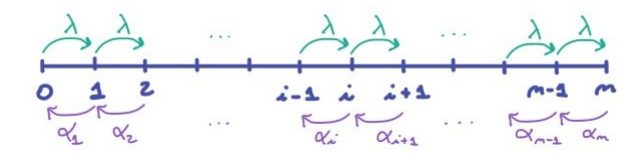
\includegraphics[width=0.75\textwidth]{diagrama_de_las_tasas_de_transicion}
\end{center}
para ciertos valores $\alpha_1, \alpha_2, \dots, \alpha_n$.
\begin{enumerate}[ref=\theexercise.\labelenumi]
	\item Mostrar que \(\alpha_i = i \mu\) para todo \(1 \leq i \leq n\).
	\item Escribir la matriz de tasas de transición \(Q\) y la matriz de probabilidades de transición asociadas.
	\item Supongamos que \(X_0 = k\) a.s., con \(k \in \{0, 1, \dots, n - 1\}\) (es decir, a tiempo inicial hay \(k\) servidores ocupados).
	\begin{enumerate}[label= \roman*., ref=\theexercise.\labelenumi.\labelenumii]
		\item Hallar la probabilidad de que el primer cliente en arribar al sistema encuentre exactamente $k$ servidores ocupados (es decir, que al instante en el que arriba el primer cliente, el proceso $\markovProcess$ pase de $k$ a $k + 1$).
		\item Hallar la probabilidad de que el primer cliente en arribar al sistema encuentre exactamente $i$ servidores ocupados, con $i \in \{0, 1, \dots, k\}$.
		(Pensar primero el caso $i = k - 1$, $i = k - 2$, ect.)
		\item Hallar el número esperado de servidores ocupados que encuentra el primer cliente que arriba al sistema.
	\end{enumerate}
\end{enumerate}
\end{exercise}

\begin{proof} \textit{a})
Supongamos que el proceso se encuentra en un estado \(i \in \{1, \dots, n\}\).
Por definición, el proceso saltará al estado \(i - 1\) siguiendo a un reloj \(T \sim \Exponential(\alpha_i)\).

Encontrarse en el estado \(i\) equivale a que \(i\) de los \(n\) servidores que forman el sistema se encuentren ocupados atendiendo a un cliente.
Visto de esta manera, el cambio del estado \(i\) al estado \(i - 1\) se dá cuando uno de los \(i\) servidores ocupados finaliza su tarea.
Luego, el cambio del estado \(i\) al estado \(i - 1\) depende de la competencia entre estos servidores.
El tiempo que tarda el \(h\)--ésimo servidor ocupado en liberarse es una variable aleatoria \(T_h \sim \Exponential(\mu)\);
y el tiempo que transcurre hasta que uno de ellos lo hace es \(\min \{T_1, \dots, T_i\}\).
En particular se sigue \(T = \min \{T_1, \dots, T_i\}\)
Nuestras hipótesis dicen que \(T_1, \dots, T_i\) son mutuamente independientes.
Entonces \(T \sim \Exponential(i \mu)\), porque la tasa del mínimo es la suma de las tasas para una familia finita e independiente de distribuciones exponenciales.

La identidad \(\alpha_i  = i \mu\) se sigue de \(T \sim \Exponential(\alpha_i)\) y \(T \sim \Exponential(i \mu)\).
\end{proof}
% \begin{}
% Supongamos que el proceso se encuentra en un estado \(i \in \{1, \dots, n - 1\}\).
% Es decir que de los \(n\) servidores que forman el sistema, \(i\) de ellos se encuentran ocupados atendiendo a un cliente y \(n - i\) estan ociosos.
% Desde este estado, el proceso puede saltar al estado \(i + 1\) o al estado \(i - 1\).
% Saltará al estado \(i + 1\) respondiendo a la llegada de un nuevo cliente.
% Y saltará al estado \(i - 1\) cuando uno de los servidores ocupados finalice su tarea.
% Luego, el cambio partiendo del estado \(i\) depende de la competencia entre \(i + 1\) relojes exponenciales.
% Uno de estos relojes, \(R \sim \Exponential(\lambda)\), describe la llegada de nuevos clientes al sistema, y suena a tasa \(\lambda\).
% Los demás \(i\) relojes, \(T_i \sim \Exponential(\mu)\) describen los tiempos de duración de las tareas que se encuentran ejecutando los \(i\) servidores activos, y suenan a tasa \(\mu\).
% Por hipótesis todos estos relojes son independientes entre sí.
% Entonces, por las propiedades particulares de las ditribuciones exponenciales, la variable \(\min (T_1, \dots, T_i, R)\) tiene distribución exponencial y su tasa es la suma de las tasas de los relojes \(T_1, \dots, T_i, R\).
% Es decir que el 
% \end{}
\begin{proof}[Cálculo] \textit{b})
Sea \(Q = (q_{i j})_{0 \leq i, j \leq n}\) la matriz generadora del proceso.
Por la definición del proceso mediante el diagrama de las tasas de transición, sabemos que \(Q\) es
\begin{align}
	\begin{pmatrix}
		- \lambda & \lambda \\
		\alpha_1 & -(\lambda + \alpha_1) & \lambda \\
		 & \alpha_2 & -(\lambda + \alpha_2) & \lambda \\
		 & & \ddots & \ddots & \ddots \\
		 & & & \alpha_{n - 2} & -(\lambda + \alpha_{n - 2}) & \lambda \\
		 & & & &\alpha_{n - 1} & -(\lambda + \alpha_{n - 1}) & \lambda \\
		 & & & & &\alpha_n & - \alpha_n
	\end{pmatrix}
\end{align}
Por el ejercicio 2.1., sabemos que \(\alpha_i = i \mu\) para todo \(i \in \{1, 2, \dots, n\}\).
Esto completa la descripción de la matriz \(Q\).

% Nota 7 dic. 2020 Teo de proba práctica clase 23.pdf %
%%%%%%%%%%%%%%%%%%%%%%%%%%%%%%%%%%%%%%%%%%%%%%%%%%%%%%%
% En este documento está la relación entre Q y Pi

Por su parte, la matriz de transición de probabilidad \(\Pi\) de la cadena de Markov asociada al proceso viene dada por \(\pi_{i i} = 0\) para todo \(i \in \{0, 1, \dots, n\}\) porque \(Q \neq 0\), y por \(\pi_{i j} = q_{i j} / Q_i = q_{i j} \left( \sum_{h \in S \setminus j} q_{i h} \right)^{- 1}\) para todo par \(i, j \in \{0, 1, \dots, n\}\) de estados distintos.
Para \(i = 0\), tenemos \(Q_0 = \lambda\).
Para \(i \in \{1, \dots, n - 1\}\), tenemos \(Q_i = i \mu + \lambda\).
Para \(i = n\), tenemos \(Q_n = n \mu\).
Luego \(\Pi\) es
\begin{align}
	\begin{pmatrix}
		0 & 1  \\
		\frac{\mu}{\mu + \lambda} & 0 & \frac{\lambda}{ \lambda + \mu} \\ 
		 & \frac{2 \mu}{2 \mu + \lambda} & 0 & \frac{\lambda}{\lambda + 2 \mu} \\
		 & & \frac{3 \mu}{3 \mu + \lambda} & 0 & \frac{\lambda}{\lambda + 3 \mu} \\
		 & & & \ddots & & \ddots \\
		 & & & & \frac{(n - 1) \mu}{(n - 1) \mu + \lambda} & 0 & \frac{\lambda}{\lambda + (n - 1) \mu} \\
		 & & & & & 1 & 0
	\end{pmatrix}
\end{align}
\end{proof}
\begin{proof}[Cálculo] \textit{c}) i.
Sea \(\tau \sim \Exponential(\lambda + k \mu)\) el reloj que marca el primer cambio de estado del sistema.
Si los relojes \(T_h \sim \Exponential(\mu)\) con \(h \in \{1, \dots, k\}\) registran la duración de las tareas de los \(k\) servidores que se encuentran ocupados a tiempo \(t = 0\), y el reloj \(C \sim \Exponential(\lambda)\) avisa de la llegada de un cliente, entonces \(\tau = \min \{T_1, \dots, T_k, C\}\).
El evento \([X_{\tau} = k + 1]\) en el cual el proceso \(\markovProcess\) pasa de \(k\) a \(k + 1\) cuando se produce un cambio de estado puede escribirse como \([\tau = C]\).
Para calcular la probabilidad de este, nos desvíamos a mencionar un teorema sobre distribuciones exponenciales independientes que probamos en la clase práctica número 20.

\begingroup
\newcommand{\exponentialVariable}{X}
\newcommand{\exponentialParameter}{\lambda}
\begin{theorem}
Supongamos \(\exponentialVariable_i \sim \Exponential(\exponentialParameter_i)\), para \(i \in \naturalnum\), son variables aleatorias independientes con \(\exponentialParameter = \sum_{i \in \naturalnum} \exponentialParameter_i < \infty\).
Entonces la distribución de su mínimo es exponencial con parámetro \(\exponentialParameter\)
\begin{align}
	\min_{i \in \naturalnum} \exponentialVariable_i \sim \Exponential(\exponentialParameter)
\end{align}
y la ley que determina cuál de las variables \(X_i\) alcanza este valor mínimo es la medida \((\exponentialParameter_j / \exponentialParameter)_{j \in \naturalnum}\)
\begin{align}
	\argmin_{i \in \naturalnum} X_i \sim \left( \frac{\exponentialParameter_j}{\exponentialParameter} \right)_{j \in \naturalnum}
\end{align}
\end{theorem}
\endgroup
De este teorema se sigue \(\prob[\min \{T_1, \dots, T_k, C\} = C] = \lambda / (\lambda + k \mu)\) porque las variables exponenciales \(T_1, \dots, T_k, C\) son mutuamente independientes.
Entonces la probabilidad de que el primer cliente en arribar al sistema encuentre exactamente \(k\) servidores ocupados es \(\lambda / (\lambda + k \mu)\).
\end{proof}
\begin{proof}[Cálculo] \textit{c}) ii.
% teorica22.pdf %
%%%%%%%%%%%%%%%%%
% mi salvación
Vamos a reconstruir nuestro proceso de Markov, pero esta vez de un modo distinto.
Seguiremos el trabajo realizado en la clase teórica número 22.

Consideremos dos procesos mutuamente independientes: una cadena de Markov \((Y_m)_{m \in \naturalnum_0}\) con espacio de estados \(\stateSpace\) y matriz de transición \(\Pi\); y una sucesión de variables aleatorias iid \((Z_m)_{m \in \naturalnum}\) con distribución \(\Exponential(1)\).
Para cada estado \(i \in \stateSpace\), escribimos su flujo de salida como \(f(i) = - q_{ii}\).
Como este flujo siempre es positivo, para cada \(m \in \naturalnum\) podemos definir el tiempo de espera \(\tau_m = Z_m / f(Y_{m - 1})\), y resulta que su distribución es \(\Exponential(f(Y_{m - 1}))\).
A partir de estas esperas definimos los tiempos de salto \(J_0 = 0\), \(J_m = \tau_1 + \tau_2 + \cdots + \tau_m\) para \(m \in \naturalnum\).
Utilizando estos datos recuperamos nuestro proceso de Markov a tiempo continuo usando la fórmula \(X_t = Y_m\) para \( t \in [J_m, J_{m + 1}[\).

Esta representación tiene la ventaja de desacoplar los estados y los tiempos de espera del sistema, resaltando la importancia de la matriz \(\Pi\).

Desde este punto de vista, la probabilidad de que el primer cliente en arribar al sistema encuentre \(i\) servidores ocupados puede pensarse del siguiente modo.
Los cambios en la cadena \((Y_m)_{m \in \naturalnum_0}\) dados por \(\nabla Y_m = Y_m - Y_{m - 1}\) --- que ocurren en el \(m\)--ésimo paso, a tiempo \(J_m\) --- nos indican si ha llegado un nuevo cliente: \(\nabla Y_m = 1\); o si uno de los servidores que se encontraba ocupado se ha liberado: \(\nabla Y_m = - 1\).
Luego, el instante en el que arriba el primer cliente puede escribirse como \(C = J_M\) donde \(M \in \naturalnum\) es aleatorio y viene dado por \(M = \min \{m \in \naturalnum : \nabla Y_m = 1\}\), y el estado en el que entra el sistema cuando llega el primer cliente puede escribirse como \(X_C = X_{J_M} = Y_M\) porque \(J_M \in [J_M, J_{M + 1}[\).
Por lo tanto, la probabilidad de que el primer cliente en arribar al sistema encuentre \(i\) servidores ocupados es igual a \(\prob(Y_M = i + 1)\).

Esta representación del proceso también hace evidente cuan rígido es.
De la definición de \(M\) se deduce \(\nabla Y_1 = \nabla Y_2 = \cdots = \nabla Y_{M - 1} = - 1\) (cuando esto tiene sentido y \(M > 1\)).
A su vez de estos cambios se sigue que \(Y_M = i + 1\) implica \(Y_{M - 1} = i\), \(Y_{M - 2} = i + 1\), \(Y_{M - 3} = i + 2\), \dots, \(Y_{M - h} = i + h - 1\), \dots, \(Y_0 = i + M - 1\).
Y restringida por la condición inicial \(Y_0 = k\), la ecuación \(Y_M = i + 1\) implica \(M = k - i + 1\).

Dada esta sucesión de estados de la cadena \((Y_m)_{m \in \naturalnum_0}\), hacemos uso de su propiedad de Markov y de la estacionaridad de sus probabilidades de transición --- \(\Pi\) no depende de \(m \in \naturalnum_0\) --- para calcular la probabilidad de \([Y_M = i + 1]\).
Para ser precisos escribimos \(\prob_k = \prob(\placeholderParameter \mid X_0 = k) = \prob(\placeholderParameter \mid Y_0 = k)\) y similar para los demás estados.
Así
\begin{align}
	&\prob_k(Y_M = i + 1) 
	\\
	&=
		\prob_k(Y_1 = k - 1, Y_2 = k - 2, \dots, Y_{k - i} = i, Y_{k - i + 1} = i + 1)
	\\
	&=
		\prob_k(Y_1 = k - 1, Y_2 = k - 2, \dots, Y_{k - i} = i) \times \prob_i(Y_1 = i + 1)
	\\
	&=
		\prob_k(Y_1 = k - 1) \prob_{k - 1}(Y_1 = k - 2) \cdots \prob_{i + 1}(Y_1 = i) \times \prob_i(Y_1 = i + 1)
\end{align}
Expresada en términos de la matriz de transición de probabilidad \(\Pi \! = \! (\pi_{a b})_{a,b \in \stateSpace}\), esta igualdad se lee
\begin{align}
	\prob_k(Y_M = i + 1)
	&=
		\pi_{k, k - 1} \pi_{k - 1, k - 2} \cdots \pi_{i + 1, 1} \times \pi_{i, i + 1}
		\\
	&= 
		\frac{k \mu}{k \mu + \lambda} \frac{(k - 1) \mu}{(k - 1) \mu + \lambda} \cdots \frac{(i + 1) \mu}{(i + 1) \mu + \lambda} \times \frac{\lambda}{\lambda + i \mu}
	\\
	&= 
		\frac{k!}{i!} \frac{ \mu}{k \mu + \lambda} \frac{\mu}{(k - 1) \mu + \lambda} \cdots \frac{\mu}{(i + 1) \mu + \lambda} \times \frac{\lambda}{\lambda + i \mu}
	\\
	&= 
		\frac{k!}{i!} \frac{1}{k + \lambda / \mu} \frac{1}{(k - 1) + \lambda / \mu} \cdots \frac{1}{i + \lambda / \mu} \times \frac{\lambda}{\lambda + i \mu}
	\\
	&= 
		\frac{k!}{i!} \frac{1}{(k + \lambda / \mu)^{\underline{i}}} \frac{\lambda}{\lambda + i \mu}
	\\
	&= 
		\frac{k^{\underline{i}}}{(k + \lambda / \mu)^{\underline{i}}} \frac{\lambda}{\lambda + i \mu}
\end{align}

Por lo tanto, la probabilidad de que el primer cliente en arribar al sistema encuentre exactamente \(i\) servidores ocupados es \(\displaystyle \frac{k^{\underline{i}}}{(k + \lambda / \mu)^{\underline{i}}} \frac{\lambda}{\lambda + i \mu}\).
\end{proof}
%%%%%%%%%%%%%%%%%%%%%%%%%%%%%
\begin{proof}[Cálculo] \textit{c}) iii.
% mi intuición me dice que es algo del optional stopping
% mi segunda hipótesis es que sale variando el estado inicial y encontrando una relación entre las distintas esperanzas.
Sea \(\Expectation_h\) la esperanza determinada por la medida \(\prob_k\).
Definamos como \(O\) al estado del sistema previo a la llegada del primer cliente.
Siguiendo los razonamientos del ejercicio anterior, puede decirse que \(O = Y_{M - 1}\).
Eso hace de \(O\) una variable aleatoria medible según la \(\sigma\)--álgebra de la cadena \((Y_m)_{m \in \naturalnum_0}\), y permite determinar el valor de \(O\) usando los caminos trazados por \((Y_m)_{m \in \naturalnum_0}\).
Escribamos \(e_h = \Expectation_h(O)\), \(h \in \{0, 1, \dots, n\}\), para analizar estos valores como una sucesión.
Al final, calcularemos estas esperanzas de forma indirecta resolviendo una relación de recurrencia.
Como valores de borde tenemos \(e_0 = 0\) por un lado y \(e_n = e_{n - 1}\) por el otro.
La primera ecuación se debe a que cuando el estado inicial del sistema tiene a todos los servidores ociosos la única posibilidad de cambio es la llegada de un cliente, y al llegar este al sistema encontrará 0 servidores ocupados.
La segunda ecuación se debe a la propiedad de Markov de la cadena \((Y_m)_{m \in \naturalnum_0}\), y a que \(\pi_{n, n - 1} = 1\).
Estas dos informaciones nos permiten deducir \(\Expectation_n(O) = \Expectation_{n - 1}(O) \pi_{n, n - 1} = \Expectation_{n - 1}(O)\).
En los casos intermedios sucede lo siguiente.
Fijamos \(h \in \{1, 2, \dots, n - 1\}\).
Descomponemos \(e_h\) en una suma de dos términos
\begin{align}
	\Expectation_h(O)
	&=
	\Expectation_h(O \characteristic_{Y_1 = h + 1})
	+ \Expectation_h(O \characteristic_{Y_1 = h - 1})
\end{align}
En el evento que \(Y_0 = h, Y_1 = h + 1\), sucede que \(O = h\).
Entonces 
\begin{align}
	\Expectation_h(O \characteristic_{Y_1 = h + 1}) 
	= 
	\Expectation_h(h \characteristic_{Y_1 = h + 1}) 
	= 
	h \prob_h(Y_1 = h + 1) 
	= 
	h \pi_{h, h + 1}
\end{align}
Por otro lado, si desagregamos el segundo término usando la propiedad de Markov y la estacionaridad de \(\Pi\)
\begin{align}
	&\Expectation_h(O \characteristic_{Y_1 = h - 1}) 
	\\
	&= 
		\sum_{o = 0}^{h - 1} o \cdot \prob_h(Y_1 = h - 1, Y_2 = h - 2, \dots, Y_{h - o} = o, Y_{h - o + 1} = o + 1)
	\\
	&=
		\sum_{o = 0}^{h - 1} o \cdot \prob_h(Y_1 = h - 1) \prob_{h - 1}(Y_1 = h - 2, \dots, Y_{h - o - 1} = o, Y_{h - o} = o + 1)
	\\
	&=
		\prob_h(Y_1 = h - 1)
	\\
		&\hspace{1em} \times \sum_{o = 0}^{h - 1} o \cdot \prob_{h - 1}(Y_1 = h - 2, \dots, Y_{h - o - 1} = o, Y_{h - o} = o + 1)
	\\
	&=
		\prob_h(Y_1 = h - 1) \Expectation_{h - 1}(O)
	\\
	&=
		\pi_{h, h - 1} e_{h - 1}
\end{align}

Por lo tanto \(e_h = e_{h - 1} \pi_{h, h - 1} + h \pi_{h, h + 1}\).
Es decir
\begin{align}
	e_h = e_{h - 1} \frac{\mu}{\lambda / h + \mu} + \frac{\lambda}{\lambda / h + \mu}
\end{align}
Esta fórmula nos permite calcular las esperanzas que queríamos.
\end{proof}
\endgroup
%%%%%%%%%%%%%%%%%%%%%%%%%%%%%%
\newpage
\begingroup
\newcommand{\brownianProcess}{(\brownian_t)_{t \geq 0}}
\newcommand{\reflectedBrownian}{\widetilde{\brownian}}
\newcommand{\wienerProcess}{(\wiener_t)_{t \geq 0}}
\begin{exercise}
Sea $\brownianProcess$ un Movimiento Browniano Estándar (abreviado MBE) en dimensión 1.

Para cada $x \in \realnum$ sea $T_x = \inf \{t \geq 0 : \brownian_t = x\}$.
(Notar que \(T_0 = 0\) a.s.)
Denotamos con \(f_{T_x}\) y \(F_{T_x}\) a la función de densidad y a la función de distribución acumulada de \(T_x\), respectivamente.
\begin{enumerate}[label=\alph*), ref=\theexercise.\labelenumi]
	\item \label{exercise:3.a)} 
	Probar que \(\prob(T_x < + \infty) = 1\) para todo \(x \in \realnum\).
	(Sugerencia: puede ser útil observar el \(\sup_{t \geq 0} \brownian_t\) y el \(\inf_{t \geq 0} \brownian_t\))
	\item \label{exercise:3.b)}
	Probar que \(\prob(T_x \leq t) = \prob(\abs{\brownian_t} \geq \abs{x}) = 2 - 2 F_{\brownian_1} \left( \abs{x} / \sqrt{t} \right)\) para todo \(x \in \realnum\) y para todo \(t \geq 0\).
	(Sugerencia: Principio de Reflexión)
	\item 
	\label{exercise:3.c)}
	Para cada \(x \in \realnum \setminus \{0\}\), calcular \(f_{T_x}\) y verificar que \(\Expectation(T_x) = + \infty\).
\end{enumerate}
\end{exercise}
\begin{proof} \ref{exercise:3.a)}
Queremos estudiar los valores que toma el movimiento browniano en un tiempo finito.
Por eso definimos, para cada \(t \in [0 , + \infty[\), un conjunto aleatorio \(V [0, t] = \{X_s : s \in [0, t]\}\).
La continuidad de las trayectorias del MBE, y el teorema de los valores intermedios, hacen de \(V [0, t]\) un intervalo cerrado: \(V [0, t] = [\sup_{0 \leq s \leq t} \brownian_s, \inf_{0 \leq s \leq t} \brownian_s]\).

Luego, para entender los valores que toma el movimiento browniano debemos estudiar sus valores extremos aleatorios \(S_t = \sup_{0 \leq s \leq t} \brownian_s\) e \(I_t = \inf_{0 \leq s \leq t} \brownian_s\).
Ahora bien, porque estos valores extremos son funciones monótonas de \(t\), el comportamiento de estas variables para a tiempos avanzados de la evolución del proceso está dado por sus límites puntuales.
Los supremos \(S_t\) convergen a \(S^* = \sup_{s \geq 0} \brownian_s\) cuando \(t \rightarrow \infty\); los ínfimos \(I_t\) convergen a \(I^* = \inf_{s \geq 0} \brownian_s\) cuando \(t \rightarrow \infty\).

En la Propiedad 5 probada en las notas sobre el Movimiento Browniano encontramos:
% Notas Movimiento Browniano.pdf %
%%%%%%%%%%%%%%%%%%%%%%%%%%%%%%%%%%
\begin{property}[5]
Sea \(\brownianProcess\) el Movimiento Browniano Estándar en \(\realnum\).
Sea \(S^* = \sup_{t \geq 0} \brownian_t\), \(I^* = \inf_{t \geq 0} \brownian_t\).
Entonces \(S^* = + \infty\) e \(I^* = - \infty\) a.s.
\end{property}
Se sigue que existe un evento \(E \subseteq \Omega\) con probabilidad total \(\prob(E) = 1\) tal que \(S^*(\omega) = + \infty\), \(I^*(\omega) = - \infty\) para todo \(\omega \in E\).
Fijando \(\omega \in E\), se verifican los límites 
\begin{align}
	&\lim_{t \rightarrow \infty} S_t(\omega) 
		= S^*(\omega) 
		= + \infty
	&
	&\lim_{t \rightarrow \infty} I_t(\omega) 
		= I^*(\omega) 
		= - \infty
\end{align}
Encontramos que para todo \(x \in \realnum\) existe \(t_x > 0\) tal que \(S_{t_x}(\omega) > x\) e \(I_{t_x}(\omega) < x\).
Luego \(x \in [I_{t_x}(\omega), S_{t_x}(\omega)] = V [0, t_x]\) y existe \(t*_x \in [0, t_x]\) tal que \(X_{t^*_x}(\omega) = x\).
Por lo tanto \(T_x(\omega) \leq t_x < \infty\) para todo \(x \in \realnum\) y para todo \(\omega\) en un evento de probabilidad total.
\end{proof}
%%%%%%%%%%%%%%%%%%%
\begin{proof} \ref{exercise:3.b)}
La Propiedad 1.\textit{i}) de las notas sobre el Movimiento Browniano dice
% Notas Movimiento Browniano.pdf %
%%%%%%%%%%%%%%%%%%%%%%%%%%%%%%%%%%
\begin{property}[1.\textit{i}]
\label{NotasMovimientoBrowniano_property:1.i)}
Sea \((\brownian_t)_{t \geq 0}\) un movimiento Browniano estándar en \(\realnum^d\).
A partir de este definimos \(\wienerProcess = (A \brownian_t)_{t \geq 0}\) con \(A \in \realnum^{n \times n}\) matriz ortogonal (o sea \(A \transpose{A} = \identity\)).
Entonces, el proceso \(\wienerProcess\) es MBE en \(\realnum^d\).
En particular, eligiendo \(A = - \identity\) nos queda que \((- \brownian_t)_{t \geq 0}\) es MBE.
\end{property}
Para nosotros es importante su corolario, según el cual las leyes que rigen a \(\brownianProcess\) y a \((- \brownian_t)_{t \geq 0}\) son idénticas.
De este se siguen \(\prob(T_x \leq t) = \prob(T_{\abs{x}} \leq t)\) y \(\prob(\abs{\brownian_t} \geq \abs{x}) = 2 \prob(\brownian_t \geq \abs{x})\).
El caso no trivial \(x < 0\) de la primera ecuación se satisface porque el corolario implica
\begin{align}
	\prob(\inf\{s : \brownian_s = x\} \leq t)
	&=
	\prob(\inf\{s : - \brownian_s = \abs{x}\} \leq t)
	\\
	&=
	\prob(\inf\{s : \brownian_s = \abs{x}\} \leq t)
\end{align}
La segunda ecuación es verdadera porque la identidad de las leyes y la continuidad absoluta de la variable \(\brownian_t \sim \normal (0, t)\) que se deriva de la definición del MBE implican
\begin{align}
	\prob(\abs{\brownian_t} \geq \abs{x})
	&=
	\prob(\brownian_t \geq \abs{x}) + \prob(- \brownian_t \geq \abs{x})
	\\
	&= 
	\prob(\brownian_t \geq \abs{x}) + \prob(\brownian_t \geq \abs{x})
\end{align}
Juntas, ambas consecuencias de la invarianza por rotaciones de la familia de los MBE nos sugieren fijar \(y = \abs{x}\) y probar la igualdad
\begin{align}
	\prob(T_y \leq t)
	=
	2 \prob(\brownian_t \geq y)
\end{align}

% Este párrafo merece un dibujito 
Pensando que las trayectorias que han alcanzado el valor \(y\) antes de tiempo \(t\) se parten en dos partes iguales según superen o no el valor \(y\) a tiempo \(t\), resaltamos la ecuación
\begin{align}
	\prob(T_y \leq t)
	&=
	\prob(T_y \leq t, \brownian_t \geq y) + \prob(T_y \leq t, \brownian_t < y)
\end{align}
La continuidad de las trayectorias del MBE \(\brownianProcess\) hace que, al comenzar en \(\brownian_0 = 0\) y superar a \(y \geq 0\) al llegar a \(\brownian_t \geq y\), necesariamente se alcance el valor \(y\) en el intervalo de tiempo \([0, t]\).
Luego \(\prob(T_y \leq t, \brownian_t \geq y) = \prob(\brownian_t \geq y)\).
Esta misma continuidad implica que alcanzar el valor \(y \geq 0\) antes de tiempo \(t\) es equivalente a que el supremo \(S_t\) supere al valor \(y\).
Luego \(\prob(T_y {\leq} t, \brownian_t {<} y) = \prob(S_t {\geq} t, \brownian_t {<} y)\).
Por otro lado, la continuidad absoluta de la variable \(\brownian_t \sim N(0, t)\) implica \(\prob(S_t \geq y, \brownian_t < y) = \prob(S_t \geq y, \brownian_t \leq y)\).
Finalmente, el Principio de Reflexión pequeño probado en las notas sobre el Movimiento Browniano nos prueba que \(\prob(S_t \geq y, \brownian_t \leq y) = \prob(\brownian_t \geq y)\).
% Notas Movimiento Browniano.pdf %
%%%%%%%%%%%%%%%%%%%%%%%%%%%%%%%%%%
\begin{corollary}[Principio de Reflexión pequeño]
\label{corollary:SmallReflectionPrincipleForBrownianMotion}
Sea \(\brownianProcess\) MBE en \(\realnum\), sean \(a, b \in \realnum\) con \(a \leq b\) y \(b > 0\).
Sea \(S_t = \sup_{0 \leq s \leq t} \brownian_s\).
Entonces, para todo \(t \geq 0\) vale que \(\prob(S_t \geq b, \brownian_t \leq a) = \prob(\brownian_t \geq 2 b - a)\).
\end{corollary}
Estas observaciones bastan para decir que
\begin{align}
	\prob(T_x \leq t)
	=
	\prob(T_y \leq t)
	=
	2 \prob(\brownian_t \geq y)
	=
	\prob(\abs{\brownian_t} \geq \abs{x})
\end{align}

Para cerrar observamos que las distribuciones de \(\brownian_t\) y de \(\sqrt{t} \brownian_1\) son idénticas porque \(\brownian_t \sim \normal(0, t)\) y \(\brownian_1 \sim \normal(0, 1)\).
En consecuencia \(2 \prob(\brownian_t \geq y) = 2 \prob \left( \brownian_1 \geq y / \sqrt{t} \right) = 2 \left(1 - \prob \left(\brownian_1 \leq y / \sqrt{t} \right)\right)\).
De aquí se desprende la fórmula \(\prob(\abs{\brownian_t} \geq \abs{x}) = 2 - 2 F_{\brownian_1} \left( \abs{x} / \sqrt{t} \right)\), donde \(F_{\brownian_1} = \PhiDistribution\) es la función de distribución acumulada de la distribución normal estándar sobre \(\realnum\).
Por las simetrías de \(\PhiDistribution\), podemos decir que \(1 - \PhiDistribution \left( \abs{x} / \sqrt{t} \right) = \PhiDistribution \left( - \abs{x} / \sqrt{t} \right)\) y concluir
\begin{align}
	\prob(T_x \leq t)
	=
	2 \PhiDistribution \left( - \frac{\abs{x}}{\sqrt{t}} \right)
\end{align}

\end{proof}
%%%%%%%%%%%%%%%%%%%%%%%%%%%%%
\begin{proof}
\ref{exercise:3.c)}
Tenemos que calcular \(f_{T_x} = \left(F_{T_x}\right)'\).
Escribimos \(\abs{x} = y\), como antes, y abreviamos \(f = f_{T_x}\), \(F = F_{T_x}\).
Por el resultado del ejercico \ref{exercise:3.b)} la función de distribución acumulada es \(F{(t)} = \prob(T_x \leq t) = 2 \PhiDistribution \left(- y / \sqrt{t} \right)\), y la función de densidad de probabilidad es \(f{(t)} = (\dd / \dd t) 2 \PhiDistribution \left(- y / \sqrt{t} \right)\).
Definimos \(\tau = y / \sqrt{t}\), y calculamos 
\begin{align}
	\frac{\dd \tau}{\dd t} 
	= 
	\frac{- y}{2 t^{3 / 2}} 
	= 
	\frac{- y^3}{2 y^2 \sqrt{t}^3}
	=
	\frac{- \tau^3}{2 y^2}
\end{align}
La regla de la cadena nos permite identificar a la función de densidad de probabilidad
\begin{align}
	f 
	= 
	2 \frac{\dd}{\dd t} \Phi(- \tau)
	=
	2 \phi(- \tau) \frac{\tau^3}{2 y^2}
	=
	\frac{\tau^3}{y^2} \phi(\tau)
\end{align}
donde \(\phi\) es la densidad de probabilidad de la distribución normal estándar en \(\realnum\) (una función simétrica en el sentido \(\phi \circ (- \identity) = \phi\)).

En cuanto a la esperanza \(\Expectation(T_x)\), esta puede calcularse como \(\int_0^{\infty} t f(t) \dd t\).
Por una parte \(t = \sqrt{t}^2 = y^2 / \tau^2\), y ya tenemos una fórmula para \(f\).
Entonces
\begin{align}
	t f(t)
	=
	\frac{y^2}{\tau^2} \frac{\tau^3}{y^2} \phi(\tau)
	=
	\tau \phi(\tau)	
\end{align}
Por otra parte, una nueva consecuencia de la regla de la cadena es
\begin{align}
	\dd t
	=
	\frac{\dd t}{\dd \tau} \dd \tau
	=
	\left( \frac{\dd}{\dd \tau} \frac{y^2}{\tau^2} \right) \dd \tau
	=
	\frac{- 2 y^2}{\tau^3} \dd \tau
\end{align}
Juntando ambas ecuaciones llegamos a
\begin{align}
	t f(t) \dd t
	=
	\tau \phi(\tau) \left( \frac{- 2 y^2}{\tau^3} \right) \dd \tau
	=
	- 2 y^2 \frac{\phi(\tau)}{\tau^2} \dd \tau
\end{align}
Si nos detenemos un momento vemos que \(\tau\) invierte el orden de \(t\), dejando \(\tau(0) = \infty\) y \(\tau(\infty) = 0\).
Por lo tanto
\begin{align}
	\int\limits_0^{\infty} t f(t) \dd t
	=
	\int\limits_{\infty}^0 - 2 y^2 \frac{\dd \tau}{\tau^2}
	=
	2 y^2 \int\limits_0^{\infty} \frac{\phi(\tau)}{\tau^2} \dd \tau
\end{align}
Esta ecuación es fatal, e implica que \(\Expectation(T_x) = \infty\).
Para probarlo, truncamos la integral de la derecha a distancia \(\varepsilon > 0\) del origen y usamos que \(\phi, \tau^{- 2}\) crecen cuando \(\tau \rightarrow 0\).
Obtenemos la cota
\begin{align}
	\int\limits_0^{\infty} \frac{\phi(\tau)}{\tau^2} \dd \tau
	\geq
	\int\limits_0^{\varepsilon} \frac{\phi(\tau)}{\tau^2} \dd \tau
	\geq
	\int\limits_0^{\varepsilon} \frac{\phi(\varepsilon)}{\varepsilon^2} \dd \tau
	\geq
	\varepsilon \frac{\phi(\varepsilon)}{\varepsilon^2}
	\geq
	\frac{\phi(\varepsilon)}{\varepsilon}
\end{align}
El límite \( \lim_{\varepsilon \rightarrow 0}\phi(\varepsilon) / \varepsilon = \infty\) puede deducirse porque \(\phi(\varepsilon) \rightarrow 1 / \sqrt{2 \pi}\) y \(1 / \varepsilon \rightarrow \infty\) cuando \(\varepsilon \rightarrow 0\).
Por lo tanto, siendo que para todo \(\varepsilon > 0\)
\begin{align}
	\Expectation(T_x)
	= 
	\int\limits_0^{\infty} t f(t) \dd t
	=
	2 y^2 \int\limits_0^{\infty} \frac{\phi(\tau)}{\tau^2} \dd \tau
	\geq
	2 y^2 \frac{\phi(\varepsilon)}{\varepsilon}
\end{align}
concluimos \(\Expectation(T_x) = \infty\).
\end{proof}
\endgroup

% \end{}
%%%%%%%%%%%%%%%%%%%%%%%%%%%%%%
\newpage
\begingroup
\newcommand{\wienerProcess}{(\wiener_t)_{t \geq 0}}
\begin{exercise}
Sea \((\brownian_t)_{t \geq 0}\) un Movimiento Browniano estándar en dimensión 1, y sean \(x > 0\), \(y > 0\).
Consideremos el stopping time \(T = T_{- y} \wedge T_x\).
\begin{enumerate}[ref=\theexercise.\labelenumi]
	\item 
	\label{exercise:4.1}
	Probar que \((\brownian_t^2 - t)_{t \geq 0}\) es una martingala.
	\item 
	\label{exercise:4.2}
	Probar que \(\Expectation(T) = xy\).
\end{enumerate}
\end{exercise}
\begin{proof} \ref{exercise:4.1}
Escribimos \(\wiener_t = \brownian_t^2 - t\), para todo \(t \geq 0\).
En tanto proceso a tiempo continuo, \((\wiener_t)_{t \geq 0}\) será una martinagala respecto a la filtración natural \((\events_t)_{t \geq 0}\) del Movimiento Browniano \((\brownian_t)_{t \geq 0}\) si
\begin{enumerate}[label=\roman*., ref=Paso \labelenumi]
	\item 
	\label{step:martingaleMeasurability}
	\(\wiener_t \in \events_t\) \((\forall\: t \geq 0)\)
	\item 
	\label{step:martingaleIntegrability}
	\(\Expectation(\abs{\wiener_t}) < \infty\) \((\forall\: t \geq 0)\)
	% Filtración aumentada del Movimiento Browniano
	% Alternar entre las sigma álgebras naturales y aumentadas puede cambiar alguna esperanza?
	% En las notas no se menciona nada en este sentido.
	%Filtración aumentada. \(\events^+_t = \bigcap_{s > t} \events^{\brownian}_s\)
	\item
	\label{step:martingaleProperty}
	\(\Expectation(\wiener_t \mid \events_s) = \wiener_s\) \((\forall\: 0 \leq s \leq t)\)
\end{enumerate}

\ref{step:martingaleMeasurability}
Para cada \(t \geq 0\), la función \(\wiener_t : \Omega \rightarrow \realnum\) puede escribirse como composión de funciones medibles
\begin{align}
	\left( \Omega, \events_t \right) 
	\xrightarrow[]{\displaystyle \quad \brownian_t \quad}
	\left( \realnum, \borel \right)
	\xrightarrow[]{\displaystyle \quad x \mapsto x^2 - t \quad}
	\left( \realnum, \borel \right)
\end{align}
Donde \(\borel = \borel(\realnum)\) es la \(\sigma\)--álgebra de Borel de \(\realnum\).
Luego, \(\wiener_t\) es medible como flecha entre los espacios \((\Omega, \events_t)\) y \((\realnum, \borel)\).

\ref{step:martingaleIntegrability}
Sea \(t \geq 0\).
Por definión de MBE la variable \(\brownian_t\) tiene ditribución \(\normal(0, t)\).
En particular tiene varianza finita \(\Variance(\brownian_t) = \Expectation(\brownian_t^2)\).
Luego
\begin{align}
	\Expectation \left( \abs{\wiener_t} \right)
	=
	\Expectation \left( \abs{\brownian_t^2 - t} \right)
	\leq
	\Expectation \left( \abs{\brownian_t^2} + t \right)
	=
	\Expectation \left( \brownian_t^2 \right) + t
	=
	\Expectation \left( \brownian_t^2 \right) + t
	<
	\infty
\end{align}

\ref{step:martingaleProperty}
Sean \(t, s\) tales que \(0 \leq s \leq t\).
Por la propiedad de los incrementos independientes incluída en la definición de MBE, sabemos que \(B_t - B_s\) es independiente de \(\events_s\).
Por eso consideramos su cuadrado
\((\brownian_t - \brownian_t)^2 = \brownian_t^2 - 2 \brownian_t \brownian_s + \brownian_s^2\) al calcular
\begin{align}
	\Expectation(\wiener_t \mid \events_s)
	&=
	\Expectation \left( \brownian_t^2 - t \mid \events_s \right)
	\\
	&=
	\Expectation \left( \brownian_t^2 \mid \events_s \right) - t
	\\
	&=
	\Expectation \left( (\brownian_t - \brownian_s)^2 + 2 \brownian_t \brownian_s - \brownian_s^2 \mid \events_s \right) - t
	\\
	&=
	\Expectation \left( (\brownian_t - \brownian_s)^2 \mid \events_s \right) 
	+ 2 \Expectation \left( \brownian_t \brownian_s \mid \events_s \right) 
	- \Expectation \left( \brownian_s^2 \mid \events_s \right) 
	- t
\end{align}

Porque \(\brownian_t - \brownian_s\) es independiente de \(\events_s\), entonces \(\Expectation \left( (\brownian_t - \brownian_s)^2 \mid \events_s \right) = \Expectation \left( (\brownian_t - \brownian_s)^2\right)\).
Por definición de MBE tenemos \(\brownian_t - \brownian_s \sim \normal(0, t - s)\).
Luego \(\Expectation \left( (\brownian_t - \brownian_s)^2\right) = \Variance(\brownian_t - \brownian_s)= t - s\).
Esto dá
\begin{align}
	\Expectation(\wiener_t \mid \events_s)
	&= 
	2 \Expectation \left( \brownian_t \brownian_s \mid \events_s \right) 
	- \Expectation \left( \brownian_s^2 \mid \events_s \right) 
	- s
\end{align}
Porque \(B_s\) es \(\events_s\)--medible (y también funciones borel medibles evaladas sobre ella, como elevar al cuadrado), sale afuera en el cálculo de las esperanzas condicionales \(\Expectation \left( \brownian_t \brownian_s \mid \events_s \right) = \brownian_s \Expectation \left( \brownian_t \mid \events_s \right)\), y \(\Expectation \left( \brownian_s^2 \mid \events_s \right) = \brownian_s^2\).
Esto dá
\begin{align}
	\Expectation(\wiener_t \mid \events_s)
	&= 
	2 \brownian_s \Expectation \left( \brownian_t \mid \events_s \right) 
	- \brownian_s^2 
	- s
\end{align}
Usando que \((\brownian_t)_{t \geq 0}\) es una martingala (como probamos en la Propiedad 3 de las notas sobre el Movimiento Browniano) llegamos al final del cálculo.
\begin{align}
	\Expectation(\wiener_t \mid \events_s)
	= 
	2 \brownian_s \Expectation \left( \brownian_t \mid \events_s \right) 
	- \brownian_s^2 
	- s
	=
	2 \brownian_s^2 - \brownian_s^2 - s
	=
	\wiener_s
\end{align}
\end{proof}
%%%%%%%%%%%%%%%%%%%%%%%%%%%%%
\begin{proof} \ref{exercise:4.2}
% Notas Movimiento Browniano.pdf %
%%%%%%%%%%%%%%%%%%%%%%%%%%%%%%%%%%
% página 11
% Corolario de propiedad de martingala del Movimiento Browniano
Hay que probar \(\Expectation(T) = xy\) con \(T = T_{- y} \wedge T_x\).
En el ejercicio \ref{exercise:4.1} probamos que \(\wiener_t = \brownian_t^2 - t\) es una martingala.
% teorica20.pdf %
%%%%%%%%%%%%%%%%%
% Teorema de los tiempos de parada 
Aplicando el teorema de los tiempos de parada a	\((\wiener^T_t)_{t \geq 0}\) y \(T = T_x \wedge T_{- y}\) tenemos que \(\Expectation(\wiener^T_T) = \).
mmmmmmmmmmmmmmmmmmmmmmmmmmmmmmmmmmmmmmmmm
\end{proof}

\endgroup
%%%%%%%%%%%%%%%%%%%%%%%%%%%%%%
\newpage
\begin{exercise}
(Este ejercicio no es obligatorio)

Sea \((B_t)_{t \geq 0}\) un Movimiento Browniano estándar en dimensión 1, y sean \(a > 0\), y \(b > 0\).
El objetivo es probar que \(\prob(B_t = a + b t \text{ para algún } t > 0) = e^{- 2 a b}\).
\begin{enumerate}[label=\alph*), ref=\theexercise.\alph*)]
	\item Sea \((X_t)_{t \geq 0}\) el proceso definido por \(X_t = e^{2 b B_t - 2 b^2 t}\).
	Probar que \((X_t)_{t \geq 0}\) es una martingala.
	\item Consideremos el stopping time \(T = \inf \{t > 0 : B_t = a + b t\}\) (donde \(T\) lo definimos como \(\infty\) si ese conjunto es vacío, es decir, si \(B_t < a + b t\) para todo \(t > 0\)).
	Probar que \(\Expectation(X_T) \characteristic_{T < \infty} = 1\).
	\item Probar que \(\Expectation(X_T \characteristic_{T < \infty}) = e^{2 a b} \prob(T < \infty)\).
	\item Concluir que \(\prob(B_t = a + b t\text{ para algún } t > 0) = e^{- 2 a b}\).
\end{enumerate}
\end{exercise}

\end{document}
